% Created 2021-10-03 Sun 13:41
% Intended LaTeX compiler: pdflatex
\documentclass[11pt]{article}
\usepackage[latin1]{inputenc}
\usepackage[T1]{fontenc}
\usepackage{graphicx}
\usepackage{grffile}
\usepackage{longtable}
\usepackage{wrapfig}
\usepackage{rotating}
\usepackage[normalem]{ulem}
\usepackage{amsmath}
\usepackage{textcomp}
\usepackage{amssymb}
\usepackage{capt-of}
\usepackage{hyperref}
\date{\today}
\title{}
\hypersetup{
 pdfauthor={},
 pdftitle={},
 pdfkeywords={},
 pdfsubject={},
 pdfcreator={Emacs 27.2 (Org mode 9.4.4)}, 
 pdflang={English}}
\begin{document}

\setcounter{tocdepth}{3}
\tableofcontents

\section*{Introduction}
\label{sec:org1510e14}

Sigma16 is a computer architecture designed for research and teaching
in computer systems.  M1 is a digital circuit that executes the Core
subset of Sigma16.  In other words, M1 is a CPU.


\begin{center}
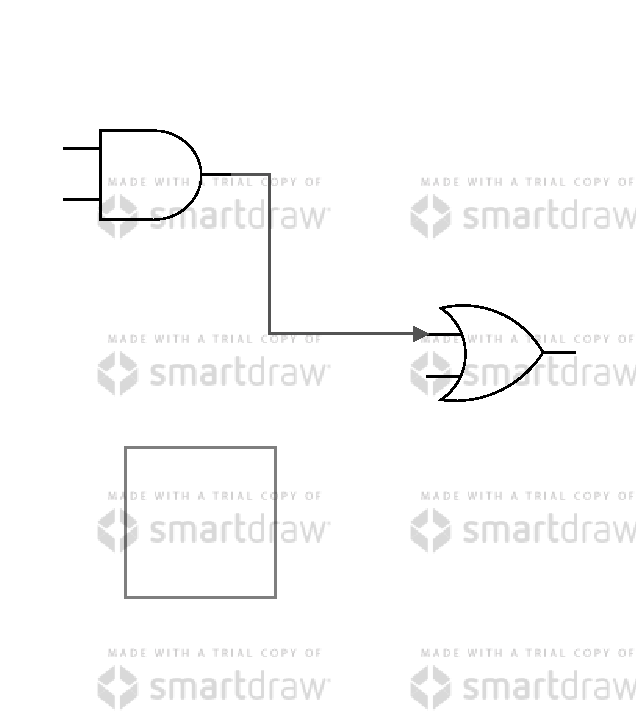
\includegraphics[width=5cm]{./figures/smartdraw-test.pdf}
\end{center}

That was a figure
\end{document}
